\section{Model\-Car\-Dyn\-Ntire  Class Reference}
\label{classModelCarDynNtire}\index{ModelCarDynNtire@{Model\-Car\-Dyn\-Ntire}}
The same model as {\bf Model2DRigid\-Dyncar\-Ntire} {\rm (p.\,\pageref{classModel2DRigidDyncarNtire})}. 


{\tt \#include $<$modelcar.h$>$}

Inheritance diagram for Model\-Car\-Dyn\-Ntire::\begin{figure}[H]
\begin{center}
\leavevmode
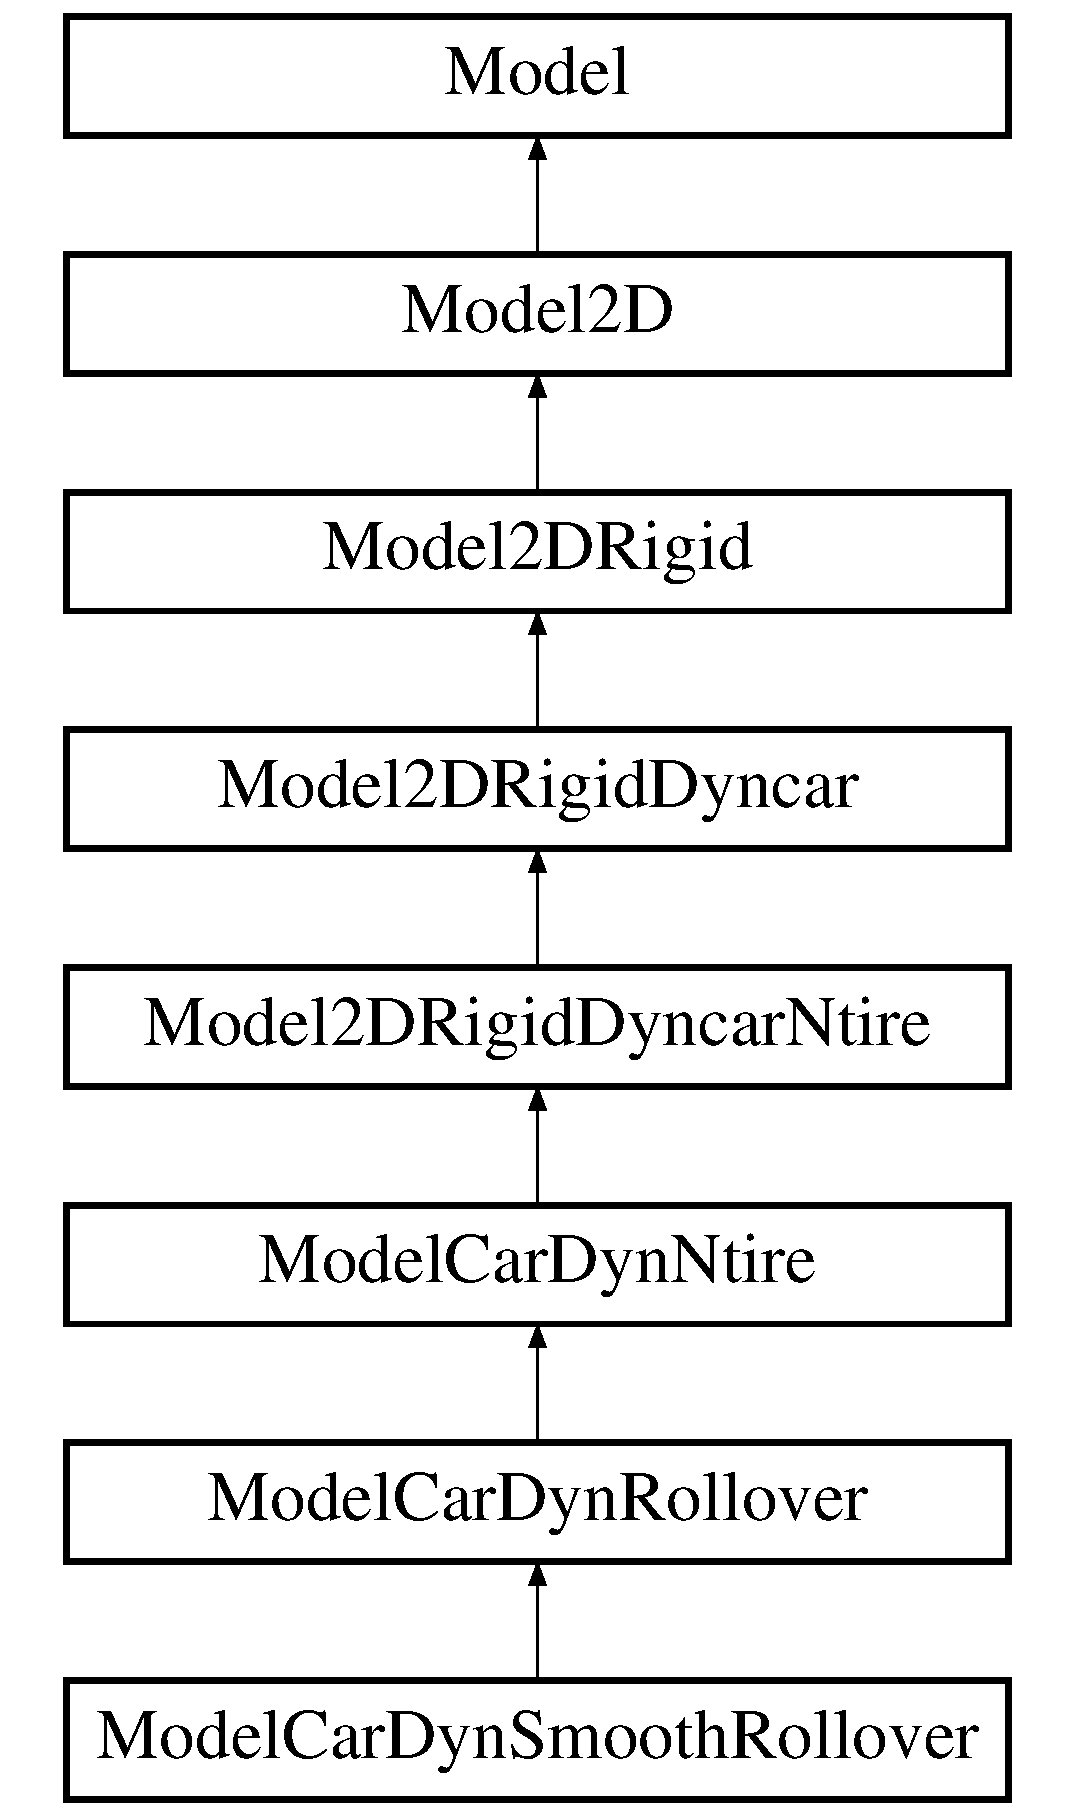
\includegraphics[height=8cm]{classModelCarDynNtire}
\end{center}
\end{figure}
\subsection*{Public Methods}
\begin{CompactItemize}
\item 
{\bf Model\-Car\-Dyn\-Ntire} (string path)
\item 
virtual {\bf $\sim$Model\-Car\-Dyn\-Ntire} ()
\item 
virtual {\bf MSLVector} {\bf State\-To\-Configuration} (const {\bf MSLVector} \&x)
\begin{CompactList}\small\item\em A method that converts a {\bf Model} {\rm (p.\,\pageref{classModel})} state in to a {\bf Geom} {\rm (p.\,\pageref{classGeom})} configuration.\item\end{CompactList}\item 
virtual double {\bf Metric} (const {\bf MSLVector} \&x1, const {\bf MSLVector} \&x2)
\begin{CompactList}\small\item\em A distance metric, which is Euclidean in the base class.\item\end{CompactList}\end{CompactItemize}


\subsection{Detailed Description}
The same model as {\bf Model2DRigid\-Dyncar\-Ntire} {\rm (p.\,\pageref{classModel2DRigidDyncarNtire})}.



\subsection{Constructor \& Destructor Documentation}
\index{ModelCarDynNtire@{Model\-Car\-Dyn\-Ntire}!ModelCarDynNtire@{ModelCarDynNtire}}
\index{ModelCarDynNtire@{ModelCarDynNtire}!ModelCarDynNtire@{Model\-Car\-Dyn\-Ntire}}
\subsubsection{\setlength{\rightskip}{0pt plus 5cm}Model\-Car\-Dyn\-Ntire::Model\-Car\-Dyn\-Ntire (string {\em path} = \char`\"{}\char`\"{})}\label{classModelCarDynNtire_a0}


\index{ModelCarDynNtire@{Model\-Car\-Dyn\-Ntire}!~ModelCarDynNtire@{$\sim$ModelCarDynNtire}}
\index{~ModelCarDynNtire@{$\sim$ModelCarDynNtire}!ModelCarDynNtire@{Model\-Car\-Dyn\-Ntire}}
\subsubsection{\setlength{\rightskip}{0pt plus 5cm}Model\-Car\-Dyn\-Ntire::$\sim$Model\-Car\-Dyn\-Ntire ()\hspace{0.3cm}{\tt  [inline, virtual]}}\label{classModelCarDynNtire_a1}




\subsection{Member Function Documentation}
\index{ModelCarDynNtire@{Model\-Car\-Dyn\-Ntire}!Metric@{Metric}}
\index{Metric@{Metric}!ModelCarDynNtire@{Model\-Car\-Dyn\-Ntire}}
\subsubsection{\setlength{\rightskip}{0pt plus 5cm}double Model\-Car\-Dyn\-Ntire::Metric (const {\bf MSLVector} \& {\em x1}, const {\bf MSLVector} \& {\em x2})\hspace{0.3cm}{\tt  [virtual]}}\label{classModelCarDynNtire_a3}


A distance metric, which is Euclidean in the base class.



Reimplemented from {\bf Model2DRigid\-Dyncar} {\rm (p.\,\pageref{classModel2DRigidDyncar_a5})}.

Reimplemented in {\bf Model\-Car\-Dyn\-Rollover} {\rm (p.\,\pageref{classModelCarDynRollover_a6})}, and {\bf Model\-Car\-Dyn\-Smooth\-Rollover} {\rm (p.\,\pageref{classModelCarDynSmoothRollover_a4})}.\index{ModelCarDynNtire@{Model\-Car\-Dyn\-Ntire}!StateToConfiguration@{StateToConfiguration}}
\index{StateToConfiguration@{StateToConfiguration}!ModelCarDynNtire@{Model\-Car\-Dyn\-Ntire}}
\subsubsection{\setlength{\rightskip}{0pt plus 5cm}{\bf MSLVector} Model\-Car\-Dyn\-Ntire::State\-To\-Configuration (const {\bf MSLVector} \& {\em x})\hspace{0.3cm}{\tt  [virtual]}}\label{classModelCarDynNtire_a2}


A method that converts a {\bf Model} {\rm (p.\,\pageref{classModel})} state in to a {\bf Geom} {\rm (p.\,\pageref{classGeom})} configuration.



Reimplemented from {\bf Model2DRigid\-Dyncar} {\rm (p.\,\pageref{classModel2DRigidDyncar_a3})}.

Reimplemented in {\bf Model\-Car\-Dyn\-Rollover} {\rm (p.\,\pageref{classModelCarDynRollover_a4})}, and {\bf Model\-Car\-Dyn\-Smooth\-Rollover} {\rm (p.\,\pageref{classModelCarDynSmoothRollover_a3})}.

The documentation for this class was generated from the following files:\begin{CompactItemize}
\item 
{\bf modelcar.h}\item 
{\bf modelcar.C}\end{CompactItemize}
